\subsection{Discriminative relational tasks}\label{ssec:experiments_discriminative}

% In this section, we study the capacity of the Abstractor to learn different kinds of relations, comparing it to existing relational architectures.

\paragraph{Order relations: modeling asymmetric relations.}

We generate $N = 64$ ``random objects'' represented by iid Gaussian vectors, $o_i \sim \mathcal{N}(0, I) \in \mathbb{R}^{32}$, and associate an order relation to them $o_1 \prec o_2 \prec \cdots \prec o_N$. Note that $\prec$ is \textit{not symmetric}. Of the $N^2 = 4096$ possible pairs $(o_i, o_j)$, 15\% are held out as a validation set (for early stopping) and 35\% as a test set. We evaluate learning curves by training on the remaining 50\% and computing accuracy on the test set (10 trials for each training set size). Note that the models are evaluated on pairs they have never seen. Thus, the models will need to generalize based on the transitivity of the $\prec$ relation.

We compare five models: an Abstractor, standard (symmetric) CoRelNet, an asymmetric variant of CoRelNet, PrediNet, and an MLP. The MLP, which is a non-relational architecture, is completely unable to learn the task. Among the relational architectures, we observe that standard CoRelNet is also completely unable to learn the task, whereas the Abstractor and asymmetric CoRelNet learn the transitive $\prec$ relation~(\Cref{fig:exp_order_relation}). PrediNet has limited success in learning the task. This can be explained by the observation that symmetric inner products (e.g., in standard CoRelNet) don't have the representational capacity to model asymmetric relations, whereas the asymmetric inner products with different learned left and right encoders do.

% This can be explained in terms of the relational bottleneck. In a relational task, there exists a sufficient statistic which is relational. The relational bottleneck restricts the search space of representations to be a space of relational features, making the search for a good representation more sample efficient. In a task in which there exists a sufficient statistic involving a \textit{symmetric} relation,
% %  (as is the case with the same/different tasks considered in~\citep{kerg2022neural}),
% we can further restrict the search space to symmetric relational representations, making learning a good representation even more sample efficient.
% However, some relations are more complex and may be asymmetric---an example is order relations. Symmetric inner products don't have the representational capacity to model such relations, but asymmetric inner products with different learned left and right encoders do.

% \subsubsection{SET: modeling multi-dimensional relations}\label{sssec:exp_set}

% might need to move this back down if we make other edits and things move around
\begin{wrapfigure}{R}{0.25\textwidth}
	\vskip-5pt
	\begin{tabular}{c}
		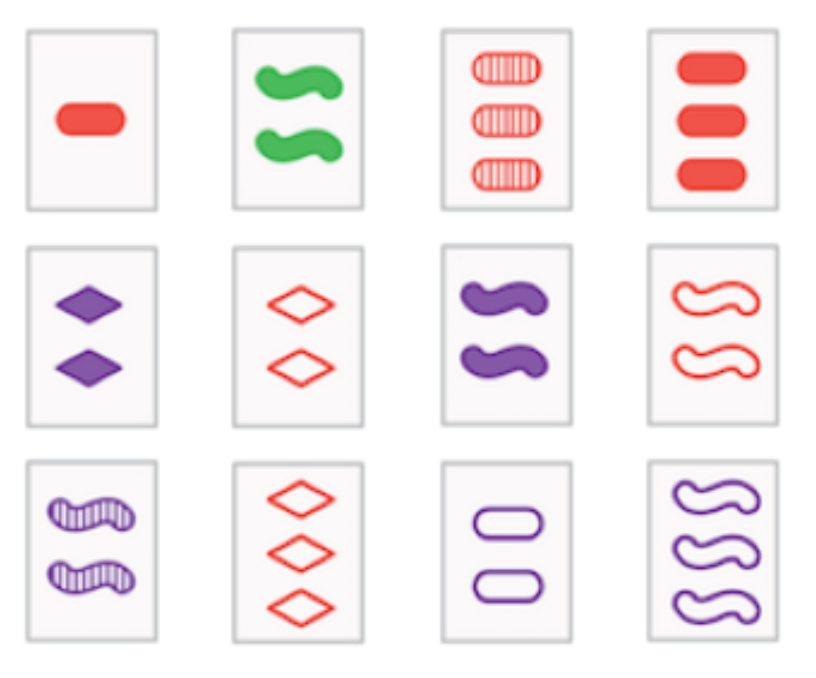
\includegraphics[width=.25\textwidth]{figures/set_example}\\[-5pt]
	\end{tabular}
	\caption{\footnotesize The SET game}\label{fig:set_example}
\end{wrapfigure}
\paragraph{SET: modeling multi-dimensional relations.}
% The $\prec$ relation is a one-dimensional relation. Similarly, the underlying relations in the experiments considered in~\citep{kerg2022neural} are also one-dimensional (same/different). In the next experiment, we explore a discriminative relational tasks which relies on a multi-dimensional relation. The task we consider is SET.
``SET'' is a cognitive task in which 
% ``SET'' is a relatively straightforward but challenging cognitive task that engages reasoning faculties in a deliberative, attentionally directed manner, requiring several levels of abstraction over sensory information. Players 
players are presented with a sequence of cards, each of which contains figures that vary along four dimensions (color, number, pattern, and shape) and they must find triplets of cards which obey a deceptively simple rule: along each dimension, cards in a `SET' must either have the same value or three unique values (\Cref{fig:set_example}). %For example, in~\Cref{fig:set_example}, the cards with two solid blue/purple diamonds, two striped blue squiggles, and two open blue oblongs form a SET: same color, same number, different patterns, different shapes.
In this experiment, the task is to classify triplets of card images as `SET' or not.

% A CNN classifier is trained on the card images to predict the four attributes. An intermediate layer is used as an embedder for all relational models. 
Again, we compare an Abstractor, CoRelNet, PrediNet, and an MLP. The shared architecture is $\texttt{CNN} \to \{\cdot\} \to \texttt{Flatten} \to \texttt{Dense}$, where $\{\cdot\}$ is one of the aforementioned modules. The CNN embedder is obtained through a pre-training task. We report learning curves in~\Cref{fig:exp_set_classification} (10 trials per training set size). We find that the Abstractor model significantly out-performs the other baselines. We attribute this to its relational inductive biases and its ability to model multi-dimensional relations. In this task, there exists four different relations (one for each attribute) which are needed to determine whether a triple of cards forms a set.
% CoRelNet would need to squeeze all of this information into a single-dimensional scalar whereas the Abstractor can model each relation separately.
We hypothesize that the ability to model relations as multi-dimensional is also part of the reason that the Abstractor is more sample efficient in learning the order relation in the previous experiment---even though the underlying relation is ``one-dimensional'', having a multi-dimensional representation enables greater robustness and multiple avenues towards a good solution during optimization.

\paragraph{SET (continued): comparison to ``neuro-symbolic'' model.}
In~\Cref{fig:set_symbolic}, to evaluate the quality of the \textit{representations} produced by Abstractors, we compare an Abstractor-based model to a ``neuro-symbolic'' model which receives as input a binary representation of the four relevant relations. We train 1-head Abstractors separately for each of the four attributes to learn same/different relations, where the task is to decide if an input pair of cards is the same or different for that attribute. We then use the $W_1$ and $W_2$ parameters learned for these relations to initialize the relations in a multi-head Abstractor. The Abstractor is then trained on a dataset of triples of cards, half of which form a SET.

This is compared to a baseline neuro-symbolic model where, instead of images, the input is a vector with 12 bits,
explicitly encoding the relations.
% That is, for each of the four attributes, a binary symbol is computed for each pair of three input cards---1 if the pair is the same in that attribute, and 0 otherwise.
A two-layer MLP is then trained to decide if the triple forms a SET. The MLP using the symbolic representation represents an upper bound on the performance achievable by any neural network model. This comparison shows that the relational representations learned by an Abstractor result in a sample efficiency that is not far from that obtained with pre-specified symbolic encodings of the relevant relations.
% This comparison shows that the Abstractor is able to solve a task using relations learned in other tasks (modularity), with a sample efficiency that is not far from that obtained with purely symbolic, noise-free encodings of the relevant relations.

% old version without comparison to symbolic MLP
% \begin{figure}[t]
%     % \vskip-.2in
%     \centering
%     \begin{subfigure}[t]{0.45\textwidth}
%         \centering
%         \vskip-20pt
%         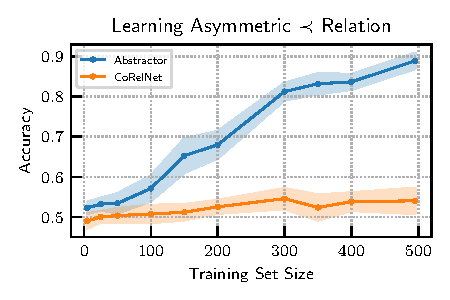
\includegraphics[width=\textwidth]{figures/experiments/pairwise_order_learning_curves.pdf}
%         \vskip-5pt
%         \caption{The $\prec$ relation can be learned with asymmetric but not symmetric inner products.}\label{fig:exp_order_relation}
%     \end{subfigure} 
%     \hskip10pt
%     % \captionsetup[subfigure]{oneside,margin={-.3in,0in}}
%     \begin{subfigure}[t]{0.45\textwidth}
%         \centering
%         \vskip-20pt
%         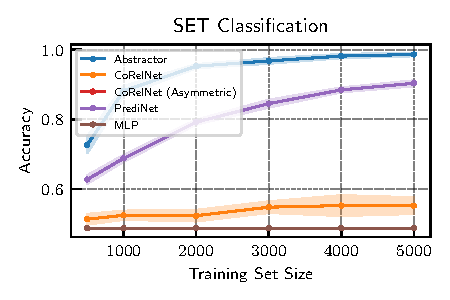
\includegraphics[width=\textwidth]{figures/experiments/set_classification.pdf}
%         \vskip-5pt
%         \caption{The Abstractor's ability to model multi-dimensional relations enables it to solve SET.}\label{fig:exp_set_classification}
%     \end{subfigure}
%     \caption{Experiments on discriminative relational tasks and comparison to CoRelNet.}
%     \vskip-15pt
% \end{figure}


\begin{figure}[t]
    % \vskip-.2in
    \centering
    \begin{subfigure}[t]{0.32\textwidth}
        \centering
        \vskip-20pt
        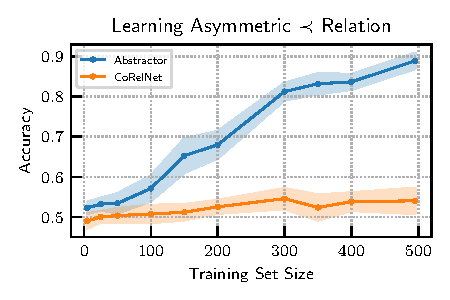
\includegraphics[width=\textwidth]{figures/experiments/pairwise_order_learning_curves.pdf}
        \vskip-5pt
        \caption{The $\prec$ relation can be learned with asymmetric but not symmetric inner products.}\label{fig:exp_order_relation}
    \end{subfigure}
    % \hskip10pt
    % \captionsetup[subfigure]{oneside,margin={-.3in,0in}}
    \begin{subfigure}[t]{0.32\textwidth}
        \centering
        \vskip-20pt
        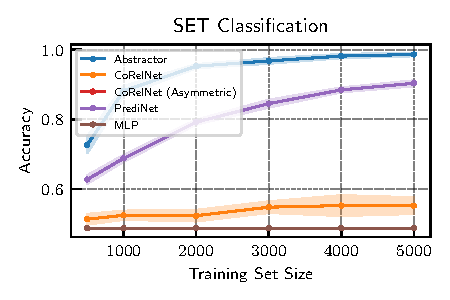
\includegraphics[width=\textwidth]{figures/experiments/set_classification.pdf}
        \vskip-5pt
        \caption{The Abstractor's ability to model multi-dimensional relations enables it to solve SET.}\label{fig:exp_set_classification}
    \end{subfigure}
    \begin{subfigure}[t]{0.32\textwidth}
        \centering
        \vskip-20pt
        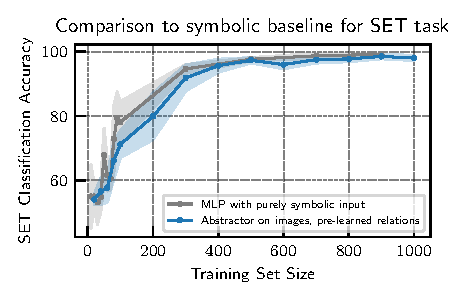
\includegraphics[width=\textwidth]{figures/experiments/set_symbolic_vs_abstractor.pdf}
        \vskip-5pt
        \caption{Comparison of Abstractor trained on card images and MLP with hand-encoded relations.}\label{fig:set_symbolic}% The Abstractor is nearly as sample 
    \end{subfigure}
    \caption{Experiments on discriminative relational tasks and comparison to CoRelNet.}
    \vskip-15pt
\end{figure}
